\documentclass[letter]{article}
\renewcommand{\baselinestretch}{1.25}

\usepackage[margin=1in]{geometry}
\usepackage{physics}
\usepackage{amsmath}
\usepackage{graphicx}
\usepackage{pythonhighlight}
\usepackage{hyperref}

\allowdisplaybreaks

%opening
\title{MECH 6327 - Homework 2}
\author{Jonas Wagner}
\date{2021, March 3}

\begin{document}

\maketitle

\newpage
\textbf{(Probably not necessary... but its long)}
\tableofcontents

\newpage
\section{Problem Set 1: Convex Sets}

\subsection{Problem 2.5}
\textbf{Problem:}\\
What is the distance between two parallel hyperplanes: $\{x \in \real^n | a^T x = b_1\}$ and $\{x \in \real^n | a^T x = b_2\}$?\\

\noindent
\textbf{Solution:}\\
Under the assumption that $a\in \real^n$ and $b_1,b_2 \in \real$, the quantity $a^T x_0$ represents the component of $x_0$ in the normal direction. Similarly, the quantities $b_1$ and $b_2$ represent the euclidean distance of the hyperplane from the origin (in the normal direction). Since the hyperplanes are parrellel, the distance between them is the difference between their offsets:
\begin{equation}
	\text{Distance between hyperplanes: } b_1 - b_2
\end{equation}


\subsection{Problem 2.7}
\textbf{Problem:}\\
\textit{Voronoi description of halfspace.} Let $a$ and $b$ be distinct points in $\real^n$. Show that the set of all points that are closer to $a$ than $b$ via the euclidean norm is a halfspace. Describe it explicitly as an inequality and draw a picture.

\noindent
\textbf{Solution:}\\
The set of all points closer to $a$ then $b$ can be defined as:
\begin{equation}
	\{x \in \real^n \ | \ \norm{x-a}_2 \leq \norm{x-b}_2\}
\end{equation}

The boundary defining this halfspace will be a plane defined by the normal vector $c$ representing the distance between $a$ and $b$, and the offset coefficient $d$ describing intersection of the plane through the half-way point between $a$ and $b$. The quantities $c$ and $d$ can therefore be defined by:
\begin{equation}
	\begin{aligned}
		c &= b - a\\
		d &= \frac{c^T a + c^T b}{2}\\
		  &= \frac{1}{2} c^T (a+b)
	\end{aligned}
\end{equation}

The halfspace, that is equivalent to $x$, can be described by the following:
\begin{equation}
	\{x\in \real^n \ | \ c^T x \leq d\}
\end{equation}

This can be visualized in two dimensions for $a = \mqty[2\\4]$ and $b = \mqty[-3\\7]$. The boundary (the red line) is calculated in the standard form using $$x_2 = \frac{-1}{c_2} \qty(c_1 * x_1 - d)$$ and then plotted. The half-space itself is the region below the boundary.

\begin{figure}[h]
	\centering
	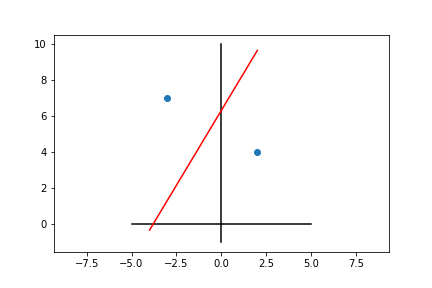
\includegraphics[width = 0.7\linewidth]{fig/pblm2_7}
	\caption{Visualization of the boundary for the halfspace.}
	\label{fig:pblm2_7}
\end{figure}


%\newpage
\subsection{Problem 2.12}
\textbf{Problem:}\\
Which of the following sets are convex?\\

\noindent
\textbf{Solution:}
\subsubsection{(a) - Slab}
A slab defined as $$\{x \in \real^n \ | \ \alpha \leq a^T x \leq \beta\}$$ \textbf{is convex} as it consists of the intersection of two halfspaces which themselves are complex.

\subsubsection{(b) - Rectangle/Hyperrectangle}
A rectangle set defined as $$\{x \in \real^n \ | \ \alpha_i \leq x_i \leq \beta_i, \ i = 1,\dots,n\}$$ \textbf{is convex} as it is composed of the intersections of half spaces which are themselves convex. This is similar to the polyhedrons/polytopes that by definition are also convex.

\subsubsection{(c) - Wedge}
A wedge set given as $$\{x \in \real^n \ | \ a_1^T x \leq b_1, a_2^T x \leq b_2\}$$ \textbf{is convex} as it is just an intersection of two halfspaces (a polyhedron).

\subsubsection{(d) - Closer to a point then a set}
A set of points closer to a given point than a given set is defined as $$\{x \| \norm{x-x_0}_2 \leq \norm{x - y}_2 \ \forall y \in S\}$$ where $S\subset\real^n$ \textbf{is not convex} in general. This is because there is not enough information about $y$ for a conclusion to be made whether it is convex or not. A counter example would be if $y$ is a point in orbit around a convex shape $S$ that would end up generating a concave $x$.

\subsubsection{(e) - Closer to a set then another set}
A set of points closer to a given set than another given set is defined as $$\{x \ | \ \textbf{dist}(x,S) \leq \textbf{dist}(x,T)\}$$ where $S, T \subset\real^n$, and $$\textbf{dist}(x,S) = \inf\{\norm{x-z}_2 \ | \ z \in S\}$$ \textbf{is not convex} in general. This is because there is not enough information about $S$ and $T$ for a conclusion to be made whether it is convex or not. A counter example includes if $S$ or $T$ themselves are a concave shave that causes the set $x$ to also be concave and therefore not convex.


\subsubsection{(f) - Set of the sum being within a convex set}
The set defined as $$\{x \ | \ x + S_2 \subseteq S_1\}$$ with $S_1$ being convex \textbf{is }\\

??????????????????????????????????????\\

\subsubsection{(g) - Set with weighted distances to two points}
The set of all points that is closer to $a$ then $b$ by at least a factor of $\theta$, defined as $$\{x \in \real^n \ | \ \norm{x-a}_2 \leq \theta \norm{x-b}_2\}$$ with $a \neq b$ and $0 \leq \theta \leq 1$ \textbf{is convex.} This is know because, as proven in a previous problem, a hyperplane is formed for a similarity stated problem which itself is convex. When the distance to $a$ must be less then a portion of the distance to $b$ it will cause the psudo-hyperplane to curve inwards and untimely remain convex.


\newpage
\subsection{Problem 2.28}
\textbf{Problem:}\\
Define the positive semi-definite cone ($S_+^n$) for $n = 1, 2, 3$ in terms of ordinary inequalities with the matrix coefficients themselves.

\noindent
\textbf{Solution:}\\
The positive semi-definite cone is defined for size $n$ as the set of all symmetric matrices that are positive semi-definite:
\begin{equation}
	S_+^n \equiv \{x \in S^n \ | \ x \succeq 0\}
\end{equation}
One method to ensure that a matrix is positive semi-definite is to ensure that its leading principle minors are all non-negative (strictly positive for positive definite).\\

For $n=1$ the required inequalities are simple, 
\begin{equation}
	X = \mqty[x_1] \in S_+^1 \iff x_1 \geq 0
\end{equation}

For $n=2$ the inequalities can be found by ensuring the leading principle minors are all non negative:
\begin{equation}
	\begin{aligned}
		m_1 &= \det[x_1]\\
		&= x_1\\
		m_2 &= \det \mqty[x_1 & x_2 \\ x_2 & x_3] \\
		&= x_1 x_3 - x_2^2
	\end{aligned}
\end{equation}
These definitions of the minors can be then be used to construct inequalities such that all the minors are positive:
\begin{equation}
	X = \mqty[x_1 & x_2 \\ x_2 & x_3] \in S_+^2 \ \iff \ \mqty{x_1 \geq 0\\  x_1 x_3 \geq x_2^2}
\end{equation}

For $n=3$ the inequalities can be found by ensuring the leading principle minors are all non negative:
\begin{equation}
	\begin{aligned}
		m_1 &= \det[x_1]\\
		&= x_1\\
		m_2 &= \det \mqty[x_1 & x_2 \\ x_2 & x_4] \\
		&= x_1 x_4 - x_2^2\\
		m_3 &= \det \mqty[x_1 & x_2 & x_3\\ x_2 & x_4 & x_5\\ x_3 & x_5 & x_6]\\
		&= x_1 (x_1 x_4 - x_2^2) - x_2 (x_2 x_6 - x_3 x_5) + x_3 (x_2 x_5 - x_3 x_4)\\
		&= x_1^2 x_4 - x_1 x_2^2 - x_2^2 x_6 + x_2 x_3 x_5 + x_2 x_3 x_5 - x_3^2 x_4
	\end{aligned}
\end{equation}
These definitions of the minors can be then be used to construct inequalities such that all the minors are positive:
\begin{equation}
	X = \mqty[x_1 & x_2 & x_3\\ x_2 & x_4 & x_5\\ x_3 & x_5 & x_6] \in S_+^2 \ \iff \ 
	\mqty{x_1 \geq 0\\
			x_1 x_4 \geq x_2^2\\
		 x_1 x_2^2 + x_2^2 x_6 + x_3^2 x_4 \geq x_1^2 x_4 + 2 x_2 x_3 x_5}
\end{equation}

\subsection{Problem 2.33}
The monotone non-negative cone is defined as all the nonnegative vectors with components sorted in non-increasing order:
\begin{equation}
	K_{m+} = \{x \in \real^n \ | \ x_1 \geq x_2 \geq \cdots \geq x_n \geq n\}
\end{equation}

\subsubsection{Part a}
\textbf{Problem:}\\
Show that $K_{m+}$ is a proper cone.

\noindent
\textbf{Solution:}\\
A set, $C \subseteq \real^n$, is considered a cone if
\begin{equation}
	\theta x \in C \ \forall x \in C \text{ and } \theta \geq 0
\end{equation}

It can be easily seen that the set $K_{m+}$ satisfies this condition as scaling each element of the matrix $x \in K_{m+}$ will equally be scaled by the same amount and the conditions of non-increasing order will still apply. This guarantees that $K_{m+}$ is in fact a cone.\\

To ensure convexity, the definition of convexity and of a cone can be incorporated into the following test:\\
The set $C \subseteq \real^n$ is a convex cone iff
\begin{equation}
	\theta_1 x_1 + \theta_2 x_2 \in C \ \forall x_1,x_2 \in C, \theta_1, \theta_2 \geq 0
\end{equation}

It is also clear that $K_{m+}$ will satisfy as if each element element of one of the matrices is scaled it maintains the nonincreasing order. The same is true for summing two $K_{m+}$ matrices as the nonincreasing order will be maintained.\\

It is also known by definition
***************************************
ask about this....


\subsubsection{Part b}
\textbf{Problem:}\\
Find the dual cone, $K_{m+}^*$.

\noindent
\textbf{Solution:}\\
A dual cone for $K$ is defined as:
\begin{equation}
	K^* = \{y \in \real^n \ | \ x^Ty \geq x^T y \geq 0 \ \forall x \in K\}
\end{equation}




?????????????????????????????????????????????????????????????????

It is known that the following is equivalent:
\begin{equation}
	\begin{aligned}
		\sum_{i=1}^{n} x_i y_i &= (x_1 - x_2) y_1 + (x_2 - x_3) (y_1 + y_2) + \cdots \\
						&= + (x_{n-1} - x_n) (y_1 + \cdots + y_{n-1}) + x_n (y_1 + \cdots + y_n)
	\end{aligned}
\end{equation}



\section{Problem Set 2: Convex Functions}

\subsection{Problem 3.6}
\textbf{Problem:}\\
What is the epigraph for the following convex functions?

\noindent
\textbf{Solution:}\\
The epigraph is defined as 
\begin{equation}
	\textbf{epi} f = \{(x,t) \ | \ x \in \textbf{dom} f, f(x) \leq t\}
\end{equation}
where $\textbf{epi} f \subset R^{n+1}$. This is equivalent to saying the space 'above' the function.

\subsubsection{(a) - Epigraph of a halfspace}
The epigraph of a halfspace in $n$ dimensions is a halfspace in $n+1$ dimensions.

\subsubsection{(b) - Epigraph of a convex cone}
The epigraph of a convex cone is another convex cone? mabye a riangular prism type thing...

\subsubsection{(c) - Epigraph of a polyhedron}
The epigraph of a polyhedron is another polyhedron. similar to convex cone... it isn't originally bounded

\subsection{Problem 3.16}
\textbf{Problem:}\\
Determine if the following functions are convex, concave, quasiconvex, or quasiconcave.

\noindent
\textbf{Solution:}\\
\subsubsection{(a) - $e^x - 1$}
Let $$f(x) = e^x - 1$$ on $\real$.\\
$f(x)$ \textbf{is convex} and can be proven in multiple ways. For instance, visualizing the epigraph of the function, it is clear that a convex set is produced. Additionally, $f(x)$ can be constructed by putting the convex function $e^x$ through the convex affine function $x - 1$.

\subsubsection{(b) - $x_1 x_2$}
Let $$f(x_1,x_2) = x_1 x_2$$ over the domain $\real_{++}^2$.\\
This function \textbf{is convex} and can be demonstrated using the definition:
\begin{align}
	f(\theta x + (1-\theta)y) &= \theta f(x) + (1-\theta) f(y)\\
	 (\theta x_1 + (1-\theta) y_1) (\theta x_2 + (1-\theta) y_2)&= \theta x_1 x_2 + (1- \theta) y_1 y_2\nonumber\\
	\theta^2 x_1 x_2 + \theta(1-\theta)y_1 x_2 + \theta (1-\theta) x_1 y_2 + (1-\theta)^2 y_1 y_2 &= \theta x_1 x_2 + (1- \theta) y_1 y_2\nonumber\\
	\theta^2 x_1 x_2 + (\theta-\theta^2) (x_1 y_2 + x_2 y_1) + (1- 2 \theta + \theta^2) y_1 y_2 &= \theta x_1 x_2 + (1- \theta) y_1 y_2
\end{align}
If we analyze each set of terms it not explicitly clear by the result, but within the domain $\real_{++}^2$ the equality holds true.\\
--------------------- add plot...

\subsubsection{(c) - $1/(x_1 x_2)$}
Let $$f(x_1,x_2) = 1/(x_1 x_2)$$ be defined over the domain $R_{++}^2$.






----------------------------------------


\subsubsection{(d) - $x_1/x_2$}
Let $$f(x_1,x_2) = x_1/x_2$$ be defined over the domain $R_{++}^2$.




----------------------------------------

\subsection{(e) - $x_1^2 / x_2$}
Let $$f(x_1,x_2) = x_1^2 / x_2$$ be defined over the domain $R \cross R_{+}$.





----------------------------------------

\subsection{(f) - $x_1^\alpha x_2^{1-\alpha}$}
Let $$f(x_1,x_2) = x_1^\alpha x_2^{1-\alpha}$$ with $0 \leq \alpha 1$ be defined over the domain $\real_{++}^2$.\\




----------------------------------------






\subsection{Problem 3.18a}
\textbf{Problem:}\\
Using the proof of concavity of the log-determinant function to show that $$f(X) = \trace(X^{-1})$$ is convex over the domain $S_{++}^n$.\\

\noindent
\textbf{Solution:}\\















\subsection{Problem 3.22}
\textbf{Problem:}\\
Use various composition rules to show that the following functions are convex.

\noindent
\textbf{Solution:}\\
\subsubsection{(a) - double log functions}
Let $$f(x) = -\log(-\log(\sum_{i=1}^m e^{a_i^T x + b_i}))$$ be defined over the domain $\{x \ | \ \sum_{i=1}^m e^{a_i^T x + b_i} < 1\}$.\\
It is known that $$\log(\sum_{i=1}^{n} e^{y_i})$$ is convex. Since all compositions of convex functions with affine functions are also convex, it can be said that $$\sum_{i=1}^m e^{a_i^T x + b_i}$$ is also convex.\\
Additionally, it is known that the $\log()$ function is concave, but when the sign changes it becomes convex, thus the composition of $-g(-g(h(x)))$ is convex for the concave function $g(x) = \log(x)$.\\
Therefore, the function $f(x)$ is convex.

\subsubsection{(b) - square root of some product sum}
Let $$f(x,u,v) = - \sqrt{uv - x^T x}$$ be defined over the domain $\{(x,u,v) \ | \ uv > x^T x, u, v > 0\}$.\\
It is known that $g(x) = x^x / u$ is convex for $u>0$ and that $h(x)-\sqrt{x_1 x_2}$ is convex on $\real_{++}^2$.\\
The function $f(x,u,v)$ can be manipulated as follows:
\begin{align*}
	f(x,u,v) 	&= - \sqrt{uv - x^T x}\\
				&= - \sqrt{u \qty(v -\cfrac{x^T x}{u})}
\end{align*}
From what we know about the underling functions, it can be said that the convex function $g(x)$ is summed with $v$ (a convex combination) and then used as an input to the convex function $h(x)$, resulting in an overall convex function.

\subsubsection{(c) - log of some product sum}
Let $$f(x,u,v) = - \log(uv - x^T x)$$ be defined over the domain $\{(x,u,v) \ | \ uv > x^T x, u, v > 0\}$.\\
It is known that $g(x) = x^x / u$ is convex for $u>0$ as well as that the $h(x) = \log(x)$ function is concave.\\
Performing the same manipulation as in the previous problem, $f(x,u,v)$ can be written as: $$f(x,u,v) = -\log(u \qty(v - \cfrac{x^Tx}{u}))$$
From this it can be derived that the convex function $g(x)$ is summed with $v$ (a convex combination) and then used as an input to the concave function $h(x)$ but is then negated to result in an overall convex function.


\subsubsection{(d) - complicated root of a powered sum and norm}
Let $$ f(x,t) = -\qty(t^p - \norm{x}_p^p)^{1/p}$$ be defined with $p>1$ over the domain $\{(x,t) \ | \ t \geq \norm{x}_p\}$.\\
It is known that $g(x,u) = \norm{x}_p^p / u^{p-1}$ is convex for $u >0$ and that $h(x,y) = -x^{1/p} y^{1 - 1/p}$ is convex over $\real_{++}^2$.

??????????????????????????????????????????????????


\subsubsection{(e) - complicated log of a powered sum and norm}
Let $$ f(x,t) = - \log(t^p - \norm{x}_p^p)$$ with $p >1$ be defined over the domain $\{(x,t) \ | \ t \geq \norm{x}_p\}$.\\
It is known that $g(x,u) = \norm{x}_p^p / u^{p-1}$ is convex for $u > 0$.



\end{document}
